% ============================================================
%  SENTINEL-GNSS — Individual Poster: Ojerinde Joel (LS2525253)
%  A1 Portrait · Compile: pdflatex (single pass)
% ============================================================
\documentclass[20pt]{extarticle}
\usepackage[T1]{fontenc}
\usepackage[utf8]{inputenc}
\usepackage{lmodern}
\usepackage[a1paper,landscape=false,
            top=1.8cm,bottom=1.8cm,left=2cm,right=2cm]{geometry}
\usepackage{multicol}
\setlength{\columnsep}{1.4cm}
\usepackage{amsmath,amssymb}
\usepackage{graphicx}
\usepackage{booktabs}
\usepackage{float}
\usepackage{caption}
\captionsetup{font=large,labelfont=bf}
\usepackage[dvipsnames]{xcolor}
\definecolor{buaaBlue}{RGB}{0,91,172}
\definecolor{buaaNavy}{RGB}{0,51,102}
\definecolor{buaaSky}{RGB}{0,160,233}
\definecolor{cleanGreen}{RGB}{76,175,80}
\definecolor{degradRed}{RGB}{244,67,54}
\definecolor{blockBG}{RGB}{235,244,252}
\usepackage{tcolorbox}
\tcbuselibrary{skins}
\usepackage{mdframed}
\usepackage{parskip}
\setlength{\parskip}{5pt}
\usepackage{enumitem}
\setlist[itemize]{noitemsep,topsep=2pt}

\newmdenv[backgroundcolor=blockBG,linecolor=buaaBlue,linewidth=2pt,
          roundcorner=6pt,innertopmargin=8pt,innerbottommargin=8pt,
          innerleftmargin=10pt,innerrightmargin=10pt,
          skipabove=6pt,skipbelow=6pt]{poblock}

\newcommand{\posec}[1]{%
  \vspace{4pt}{\large\bfseries\color{buaaNavy}#1}\\[-4pt]
  {\color{buaaBlue}\rule{\linewidth}{1.5pt}}\vspace{4pt}}

\pagestyle{empty}

\begin{document}

% HEADER
\noindent
\begin{tcolorbox}[colback=buaaNavy,colframe=buaaNavy,boxrule=0pt,arc=8pt,
                  left=16pt,right=16pt,top=10pt,bottom=10pt]
  \begin{center}
    {\fontsize{46}{54}\bfseries\color{white} SENTINEL-GNSS — Individual Poster}\\[6pt]
    {\fontsize{26}{32}\color{buaaSky}
     Architecture, Training, EKF Integration, and Documentation}\\[8pt]
    {\large\color{white}
     \textbf{Ojerinde Joel} (LS2525253) \quad
     Project Lead · Model Architect · Sensor Fusion Engineer}\\[4pt]
    {\normalsize\color{white!70!buaaSky}
     Beihang University H3I · 2025}
  \end{center}
\end{tcolorbox}

\vspace{0.5cm}

\begin{multicols}{3}

% ---- COLUMN 1 ----
\posec{My Role in the Project}
\begin{poblock}
I led the core technical pipeline of SENTINEL-GNSS:
\begin{itemize}
  \item Repository creation and code architecture
  \item 37-feature specification (\texttt{feature\_list.py})
  \item Transformer+BiLSTM neural network design \& training
  \item 9-state EKF formulation (Joseph-form covariance)
  \item SENTINEL adaptive R integration
  \item Huber robust EKF (IRLS) — calibrated for each receiver
  \item Bootstrap Particle Filter with Student-$t$ likelihood
  \item Inference packaging (0.039\,ms/sample)
  \item Dashboard backend + Huber/PF track integration
  \item All documentation and paper writing (3 docs, 5 paper sections)
\end{itemize}
\end{poblock}

\posec{Architecture I Designed}
\begin{poblock}
\textbf{Input}: $(B, 60, 37)$ feature windows

\textbf{Transformer Encoder}\\
2 layers · 4 heads · $d=128$ · $d_{ff}=512$\\
Captures: PDOP trends, satellite rise/set events

\textbf{BiLSTM}\\
2 layers · hidden\,256 (128/direction)\\
Captures: sequential C/N$_0$ decline, directional approach

\textbf{3 Output Heads}: $+5$\,s, $+15$\,s, $+30$\,s
\quad (one forward pass, 1.46\,M params)

\textbf{Training}: Focal loss $\gamma=1.0$, class weights $[1,2,5]$,\\
AdamW $10^{-3}$, cosine annealing, early stopping patience\,20
\end{poblock}

\begin{center}
  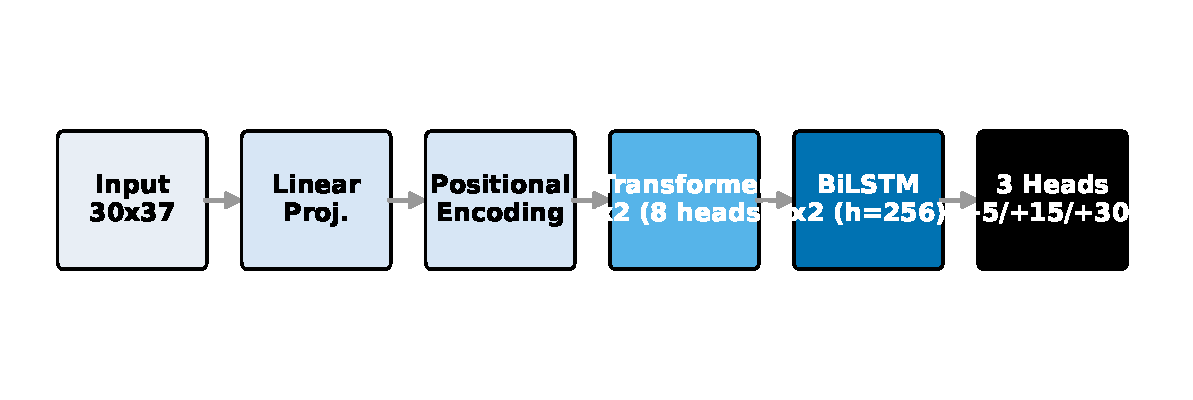
\includegraphics[width=0.95\columnwidth]{../../results/paper_figures/fig14_architecture.pdf}
  \captionof{figure}{SENTINEL-GNSS hybrid architecture.}
\end{center}

\posec{Why Hybrid? (Ablation)}
\begin{poblock}
\begin{tabular}{lcc}
  \toprule
  Architecture & Macro-F1 & DEG F1 \\
  \midrule
  Transformer-only & 0.767 & 0.571 \\
  BiLSTM-only      & 0.767 & 0.645 \\
  \textbf{Full (mine)} & \textbf{0.821} & \textbf{0.718} \\
  \bottomrule
\end{tabular}
\medskip

Transformer alone over-flags (precision 0.42).
BiLSTM alone under-recalls (recall 0.645 vs \textbf{0.847}).
Together they are complementary.
\end{poblock}

% ---- COLUMN 2 ----
\posec{SENTINEL Adaptive EKF}
\begin{poblock}
\textbf{9-state EKF}: $\mathbf{x} = [x, y, v_x, v_y, \psi, b, b_{a_x}, b_{a_y}]^\top$

At each epoch, SENTINEL $P(\text{DEGRADED})$ selects R:
\[
  \mathbf{R} = \begin{cases}
    (40\,\mathrm{m})^2\mathbf{I} & P > 0.45 \text{ (pre-emptive)} \\
    r_\mathrm{base}^2\mathbf{I}  & \text{otherwise}
  \end{cases}
\]
Kalman gain reduces \textbf{before} bad GPS arrives.
Joseph-form update for numerical stability.
\end{poblock}

\posec{Huber Robust EKF (My Design)}
\begin{poblock}
Addresses non-Gaussian GPS noise (NLOS heavy tails):

\[
  w_i = \min\!\left(1,\;\frac{c\,\tilde{\sigma}_i}{|\tilde{y}_i|}\right),
  \quad R_{ii}^H = \frac{R_{ii}}{w_i}
\]

\textbf{Key calibration insight (my finding):}\\
Threshold $= c \times r_\mathrm{base}$ must match ACTUAL GPS error scale.

\begin{tabular}{lcc}
  \toprule
  Receiver & $c$ & Threshold \\
  \midrule
  Trimble & 5.0  & 20\,m \\
  u-blox  & 30.0 & 240\,m \\
  \bottomrule
\end{tabular}

u-blox 99th-pct innovation: 208.9\,m.\\
$c=5$ (threshold 40\,m) fired on 22.7\,\% of valid updates.\\
$c=30$ fires only on the 1472\,m outlier spike. ✓

\medskip
\textbf{SENTINEL + Huber conflict:} Must run \texttt{adaptive=False}.\\
Stacking both: SENTINEL lowers gain → drift → large innovations →
Huber suppresses recovery → filter paralysis.
\end{poblock}

\posec{Particle Filter (My Design)}
\begin{poblock}
N\,=\,500 particles · Student-$t$ GPS likelihood ($\nu=3$):
\[
  \log p \propto -\tfrac{\nu+1}{2}
  \!\left[\log\!\!\left(1+\tfrac{d_x^2}{\nu r^2}\right)+
           \log\!\!\left(1+\tfrac{d_y^2}{\nu r^2}\right)\right]
\]
ESS threshold N/3 · NHC $r_\mathrm{nhc}=1.0$\,m/s\\
Jitter: $[3.0, 3.0, 0.2, 0.2, 0.05, 0.2, 0.02, 0.02]$\,m

\medskip
\textbf{GPS attractor phenomenon (my discovery):}
With persistent bias \& N=500, weight ratio climbs $1.65^5 \approx 13$
over 5 epochs → all particles cluster at biased GPS.
Needs N≥2000 or multi-hypothesis proposal to fix.
\end{poblock}

% ---- COLUMN 3 ----
\posec{Fusion Results}
\begin{poblock}
\begin{tabular}{lcc}
  \toprule
  Method / Scenario & Deg.RMSE & Gain \\
  \midrule
  EKF Fixed-R · Trimble    & \textbf{24.3\,m} & \textbf{48.8\,\%} \\
  Huber EKF · u-blox       & \textbf{58.6\,m} & \textbf{25.2\,\%} \\
  PF Student-$t$ · Odaiba  & \textbf{35.4\,m} & \textbf{40.1\,\%} \\
  \bottomrule
\end{tabular}
\end{poblock}

\begin{center}
  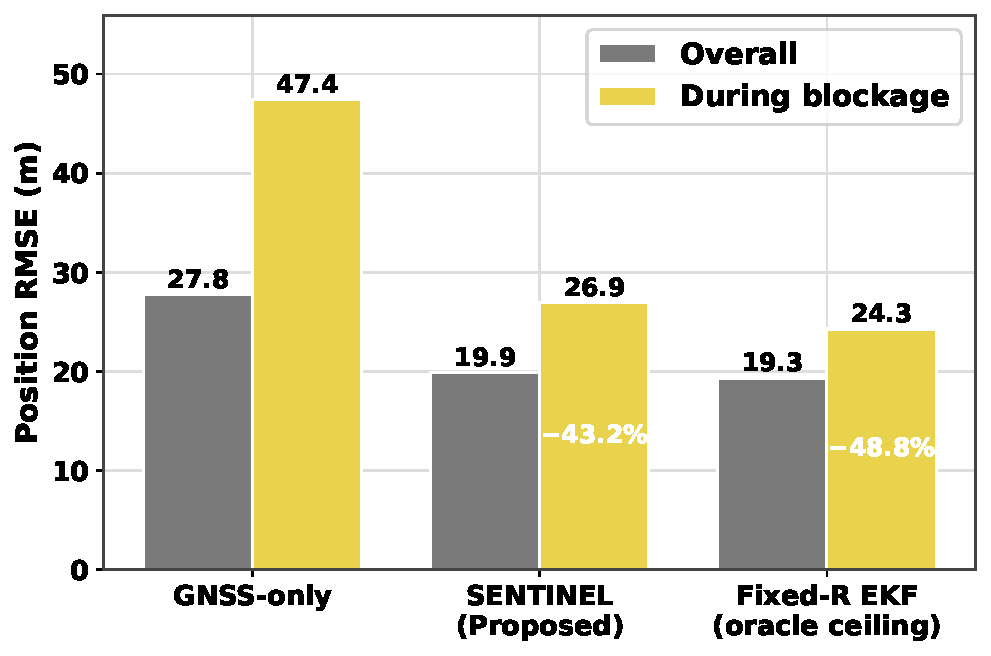
\includegraphics[width=\columnwidth]{../../results/paper_figures/fig07_ekf_rmse.pdf}
  \captionof{figure}{Degraded-segment RMSE across all methods.}
\end{center}

\posec{The ``Swirling'' Problem Solved}
\begin{poblock}
Without SENTINEL, the EKF swirls between successive NLOS GPS fixes
(each pulls the estimate off-course).

With SENTINEL pre-emptive R inflation: Kalman gain drops \emph{before}
bad GPS arrives. IMU dead-reckoning dominates the 5–30\,s NLOS window.
Trajectory stays smooth and accurate.

The vehicle's downstream controller gets a \textbf{reliable position} to act on —
which is the whole point.
\end{poblock}

\posec{Feature Saliency (My Interpretation)}
\begin{center}
  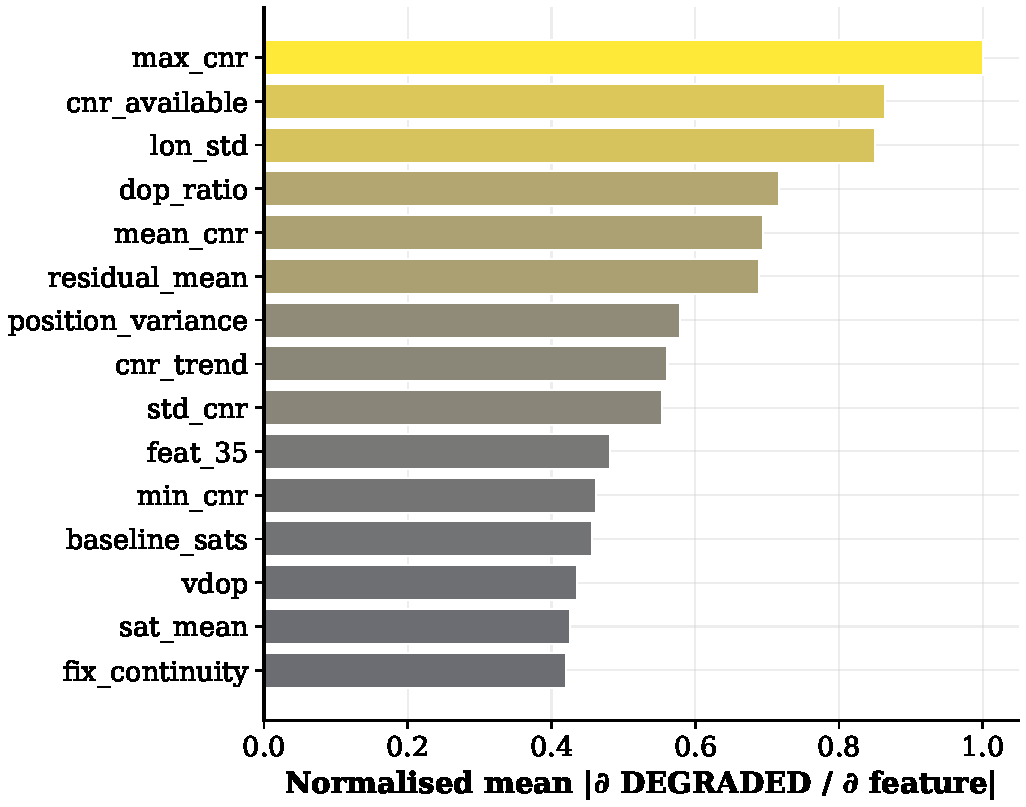
\includegraphics[width=\columnwidth]{../../results/figures/feature_saliency_5s.pdf}
  \captionof{figure}{Most important features for +5\,s prediction.
  PDOP, pseudorange residuals, and $\Delta$C/N$_0$ are top-ranked.}
\end{center}

\posec{Key Lesson}
\begin{poblock}
\textbf{Calibrate Huber $c$ to actual GPS errors, not model parameters.}
Setting $c=5$ with $r_\mathrm{base}=8$\,m gives 40\,m threshold —
fires on 22.7\,\% of valid u-blox epochs, causing drift.
Setting $c=30$ gives 240\,m threshold — fires only on the catastrophic outlier.
Result: 46.6\,m RMSE vs 88\,m with wrong $c$.
\end{poblock}

\end{multicols}

\noindent{\color{buaaBlue}\rule{\linewidth}{1.5pt}}\\[2pt]
{\small\color{buaaNavy}\centering Contact: joelojerinde@gmail.com \quad
  Beihang University H3I · 2025}

\end{document}
